% DO NOT COMPILE THIS FILE DIRECTLY!
% This is included by the other .tex files.

\begin{frame}[t,plain]
\titlepage
\end{frame}

\section{Keller-Segel model}

\begin{frame}{Keller-Segel model}
  \small
  \begin{block}{}
  \vspace*{-0.5cm}
  \begin{subequations}
      % \label{cha3:problem:KS}
      \begin{align*}
      % \label{cha3:eq:KS_u}
      \partial_t u&=\framedmath<2>{k_0\Delta u}\framedmath<3>{-k_1\nabla\cdot(u\nabla v)},\quad&\text{in }\Omega\times (0,T),\\
      % \label{cha3:eq:KS_v}
      \tau\partial_t v&=\framedmath<2>{k_2\Delta v}\framedmath<4>{-k_3v}\framedmath<4>{+k_4u},\quad&\text{in }\Omega\times (0,T),\\
      \partial_\mathbf{n}u& :=\nabla u\cdot \mathbf{n}=0,\quad
      \partial_\mathbf{n} v 
      =0, \quad &\text{on }\partial\Omega\times (0,T),\\
      % \label{cha3:eq:CI.cahn-hilliard+adveccion}
      u(0)&=u_0,\quad v(0)=v_0\text{ if }\tau>0,\quad&\text{in }\Omega.%\\
      \end{align*}
  \end{subequations}
  \end{block}
  % where $k_i>0$ for $i\in\{0,1,2,3,4\}$ and $\tau\in\{0, 1\}$ is considered to write the parabolic system when $\tau=1$, or the parabolic-elliptic for $\tau=0$.

  \begin{itemize}
      \setlength{\itemsep}{0.1em}
      % \item $u$ denotes a certain cell distribution.
      % \item $v$ stands for the concentration of
      % chemoattractant.
      \item<2> \myframed{Auto-diffusion phenomena.} %$-k_0\Delta u$ and $-k_2\Delta v$.
      \item<3> \myframed{Cross-diffusion term (migration mechanism).}%: $-k_1\nabla\cdot(u\nabla v)$.
      \item<4> \myframed{Degradation and production of chemoattractant.}%: $-k_3v$ and $k_4u$.
      \item<5> Uncontrolled aggregation
      of $u$ give rise to \structure{blowing up or exploding in finite time} (\alert{chemotactic collapse}).
  \end{itemize}
  \vspace*{-0.3cm}
  
  \uncover<6>{
  \begin{remark}
      There is a \alert{positive classical solution} of the Keller-Segel problem at least \alert{local in time}, i.e., $u, v\ge 0$ in $\Omega\times (0,T)$ whenever $u_0, v_0\ge 0$ in $\Omega$.
  \end{remark}
  }
\end{frame}

\begin{frame}{Properties of the model}
  % \begin{remark}
  %     \label{cha3:rmk:mass_conservation_KS}
  %     By taking $\bu=1$ in 
  %     \eqref{cha3:eq:KS_form_var_1} (or \eqref{cha3:eq:KS_form_var_mu_1}), any solution $u$
  %     conserves the mass, because
  %     $$\frac{d}{dt}\int_\Omega u(x,t)dx=0.$$
  % \end{remark}
  % \begin{remark}  By taking (formally) $\bu=\mu(t)$, $\bmu=\partial_t u(t)$
  %     and $\bv=(k_1/k_4)\partial_t v(t) $ 
  %     in \eqref{cha3:problem:KS_form_var_mu},
  %     and adding the resulting expressions, one has that any solution $(u,v)$
  %     satisfies the following  energy law
  %     \begin{align}
  %     \label{cha3:ley_energia_continua_KS}
  %     \frac{d }{dt}E(u(t),v(t))&+\tau\frac{k_1}{k_4}\int_\Omega |\partial_t v(t)|^2dx
  %     + \int_\Omega u(t)\left\vert\nabla(\mu(t))\right\vert^2 dx =0,
  %     \end{align}
  %     where $E\colon H^1(\Omega)_+\times H^1(\Omega)\longrightarrow\R$ is the energy functional, defined as follows
  %     \begin{align}
  %     \label{cha3:energia_KS}
  %     E(u,v)&\coloneqq\int_\Omega \left(k_0u\log(u)-k_1uv+\frac{k_1k_2}{2k_4}\vert\nabla v\vert ^2+\frac{k_1k_3}{2k_4}v^2\right),
  %     \end{align}
  %     and $H^1(\Omega)_+=\{u\in H^1(\Omega)\colon u\ge 0\}$.
  % \end{remark}
  \begin{itemize}
      \setlength{\itemsep}{1em}
      \item \structure{Mass-conservation}: $\alert{\frac{d}{dt}\int_\Omega u(x,t)dx}=0.$
      \item $\alert{u, v\ge 0}$ in $\Omega\times (0,T)$ whenever $u_0\ge 0$ and $v_0\ge0$ in $\Omega$.
      \item The following \structure{energy law} holds:
      $$
      \alert{\frac{d }{dt}E(u(t),v(t))}+\tau\frac{k_1}{k_4}\int_\Omega |\partial_t v(t)|^2dx
      + \int_\Omega u(t)\left\vert\nabla(\mu(t))\right\vert^2 dx =0,
      $$
      where
      $$
      \alert{E(u,v)}\coloneqq\int_\Omega \left(k_0u\log(u)-k_1uv+\frac{k_1k_2}{2k_4}\vert\nabla v\vert ^2+\frac{k_1k_3}{2k_4}v^2\right).
      $$

      In particular,  the energy is nonincreasing in time,
      % the solution is \structure{energy-stable} in the sense
       $$\alert{\frac{d }{dt}E(u(t),v(t))\le 0}.$$
  \end{itemize}
\end{frame}

\begin{frame}{Problem as gradient flow}
  We take, formally, the chemical potential of $u$, $$\alert{\mu}=k_0\log(u) - k_1 v.$$
  We can rewrite the problem as a gradient flow:
  \begin{block}{}
      \vspace*{-0.5cm}
      \begin{subequations}
          % \label{cha3:problem:KS}
          \begin{align*}
          % \label{cha3:eq:KS_u}
          \partial_t u&=\nabla\cdot\left(u\nabla\mu\right),\quad&\text{in }\Omega\times (0,T),\\
          \mu &= k_0\log(u)-k_1v,\quad&\text{in }\Omega\times (0,T),\\
          % \label{cha3:eq:KS_v}
          \tau\partial_t v&=k_2\Delta v-k_3v+k_4u,\quad&\text{in }\Omega\times (0,T),\\
          \partial_\mathbf{n}u& :=\nabla u\cdot \mathbf{n}=0,\quad
          \partial_\mathbf{n} v 
          =0, \quad &\text{on }\partial\Omega\times (0,T),\\
          % \label{cha3:eq:CI.cahn-hilliard+adveccion}
          u(0)&=u_0,\quad v(0)=v_0\text{ if }\tau>0,\quad&\text{in }\Omega.%\\
          \end{align*}
      \end{subequations}
      \end{block}

  We expect that, for a very small $\alert{\varepsilon}$,
  \begin{align*}
      \alert{\mu}&\simeq k_0\log(u+\alert{\varepsilon}) - k_1 v.
      % ,\\
      % \nabla\cdot\left(u\nabla\mu\right)&\simeq k_0\Delta u-k_1\nabla\cdot(u\nabla v).
  \end{align*}
\end{frame}

\subsection{Numerical approximation}

\begin{frame}{\setbeamerfont{footnote}{size=\scriptsize}Fully discrete scheme\footfullcite{acosta-soba_KS_2022}}
  \footnotesize
  Let $v^{m}\in \Pc_1(\T_h)$ and $u^{m}\in \Pd_0(\T_h)$ such that $v^m\ge 0$ in the case $\tau>0$ and $u^m\ge 0$ be given.

\begin{block}{}
\begin{subequations}
\structure{\underline{Step 1}}: Find  \alert{$v^{m+1}\in \Pc_1(\T_h)$} solving
% \label{cha3:esquema_DG_upw_KS_non_truncated}
\begin{align*}
% \label{cha3:eq:esquema_DG_upw_KS_non_truncated_1}
\tau\escalarML{\delta_tv^{m+1}}{\bv}&+k_2\escalarLd{\nabla v^{m+1}}{\nabla\bv}+k_3\escalarML{v^{m+1}}{\bv}-k_4\escalarL{u^m}{\bv}=0,
%  \forall \bv\in \Pc_1(\T_h).
\end{align*}
for all $\bv\in \Pc_1(\T_h)$.

\

\structure{\underline{Step 2}}: Find \alert{$(u^{m+1},\mu^{m+1})\in \Pd_0(\T_h)\times \Pd_0(\T_h)$} with \alert{$u^{m+1}\ge 0$} solving the coupled problem
\begin{align*}
% \label{cha3:eq:esquema_DG_upw_KS_non_truncated_2}
\escalarL{\delta_tu^{m+1}}{\bu}&+\aupw{\mu^{m+1}}{u^{m+1}}{\bu}=0,\\
% \forall \bu\in \Pd_0(\T_h)\\
% \label{cha3:eq:esquema_DG_upw_KS_non_truncated_3}
\escalarL{\mu^{m+1}}{\bmu}&-k_0 \escalarL{\log(u^{m+1}+\varepsilon)}{\bmu}+ k_1\escalarL{v^{m+1}}{\bmu}=0, 
% \forall \bmu\in \Pd_0(\T_h).
\end{align*}
for all $\bu,\bmu\in \Pd_0(\T_h)$.
\end{subequations}
% where $\aupw{\cdot}{\cdot}{\cdot}$ will be defined below in Section~\ref{cha3:sec:def_upw}.
\end{block}
\end{frame}

\begin{frame}{Assumptions on the mesh}
  \small
  \vspace*{-0.2cm}
  \begin{hypothesis}[Angles]
      \label{cha3:hyp:mesh_acute}
      The \alert{mesh $\T_h$ is acute}, i.e., the angles of the triangles of $\T_h$ are less than or equal to $\pi/2$.
  \end{hypothesis}
  \vspace*{-0.1cm}
  \begin{hypothesis}[Barycenters]
      \label{cha3:hyp:mesh_n}
      The mesh $\T_h$ of $\overline\Omega$ is structured in the sense that the \alert{line between the barycenters} of the triangles $K$ and $L$ is \alert{orthogonal to the interface} $e=K\cap L\in\E_h^i$.
  \end{hypothesis}
  \begin{figure}
      \begin{minipage}{0.5\textwidth}
          \begin{flushright}
              
\includegraphics[scale=0.5]{img/chapter3/adjacent_baricenters.pdf}
          \end{flushright}
      \end{minipage}
      \hspace*{0.5cm}
      \begin{minipage}{0.25\textwidth}
          \caption{Structure of the mesh}
      \end{minipage}
      \hfill
  \end{figure}
\end{frame}

\begin{frame}{Definition of upwind bilinear form $\aupw{\cdot}{\cdot}{\cdot}$}
  \setbeamercovered{transparent}
  \vspace*{-0.5cm}
  \begin{align*}
      % \label{cha3:def:aupw}
      \alert{\aupw{\mu}{u}{\bu}}\coloneqq& \int_\Omega (\nabla\mu\cdot\nabla\bu)u
      \\&+ \sum_{e\in\E_h^i,e=K\cap L}\int_e\left(\left(-\nabland\mu\right)_\oplus\uK-(-\nabland\mu)_\ominus\uL\right)\salto{\bu},
  \end{align*}
%   \onslide<2>{
  \only<2>{
      where, for every $e\in\E_h^i$ with $e=K\cap L$,
  \begin{equation*}
      % \label{cha3:eq:approx_gradn}
      \alert{\nabland\mu} =\frac{-\salto{\Pi_0\mu}}{\mathcal{D}_e(\T_h)}= \frac{\Pi_0\muL-\Pi_0\muK}{\mathcal{D}_e(\T_h)}.
  \end{equation*}
      % with
  \begin{minipage}{0.68\textwidth}
    \begin{itemize}
        \setlength{\itemsep}{0.5em}
        \item $\alert{\Pi_0}$ 
        % is the 
        projection on $\Pd_0(\T_h)$.
        \item $\alert{\mathcal{D}_e(\T_h)}$ 
        % is the 
        distance between 
        % the 
        barycenters $C_K$ and $C_L$ with $e=K\cap L$.
        % of the triangles $K$ and $L$ of the mesh $\T_h$ that share $e\in\Ehi$.
        \item $\alert{\nabland\mu}$ 
        % is the 
        slope of the line between $(C_K, \mu(C_K))$ and $(C_L,\mu(C_L))$, parallel to $\nn_e$.
    \end{itemize}
  \end{minipage}
  }
  \hfill
  \begin{minipage}{0.25\textwidth}
    \vspace*{-0.2cm}
    \begin{figure}
        \centering
        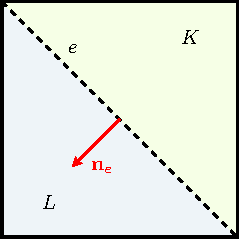
\includegraphics[width=0.75\textwidth]{img/orientation_n.pdf}
        \caption{Orientation of the mesh}
    \end{figure}
  \end{minipage}

\end{frame}

% \begin{frame}{Auxiliary truncated scheme}
%   \begin{block}{}
%       \vspace*{-0.1cm}
%   \begin{subequations}
%       % \label{cha3:esquema_DG_upw_KS_truncated}
%       \structure{\underline{Step 1}}: Given $v^m\in\Pc_1(\T_h)$ such that $v^m\ge 0$ in the case $\tau >0$, find  $v^{m+1}\in \Pc_1(\T_h)$ solving
%       \begin{align*}
%       % \label{cha3:eq:esquema_DG_upw_KS_truncated_v}
%       \tau\escalarML{\delta_tv^{m+1}}{\bv}&+k_2\escalarLd{\nabla v^{m+1}}{\nabla\bv}+k_3\escalarML{v^{m+1}}{\bv}-k_4\escalarL{u^m}{\bv}=0,
%       \end{align*}
%       for all $\bv\in \Pc_1(\T_h)$.
  
%       \
      
%       \structure{\underline{Step 2}}:  Given $u^m, \mu^m\in\Pd_0(\T_h)$ such that $u^m\ge 0$, find $u^{m+1},\mu^{m+1}\in \Pd_0(\T_h)$ solving
%       \begin{align*}
%       % \label{cha3:eq:esquema_DG_upw_KS_truncated_u}
%       \escalarL{\delta_tu^{m+1}}{\bv}&+\aupw{\mu^{m+1}}{\alert{(u^{m+1})_\oplus}}{\bu}=0,\\
%       % \label{cha3:eq:esquema_DG_upw_KS_truncated_mu}
%       \escalarL{\mu^{m+1}}{\bmu}&-k_0 \escalarL{\log(u^{m+1}+\varepsilon)}{\bmu}+ k_1\escalarL{v^{m+1}}{\bmu}=0,
%       \end{align*}
%       for all $\bu,\bmu\in \Pd_0(\T_h)$. 
%   \end{subequations}
%   \end{block}
% \end{frame}

\begin{frame}{Properties of the 
  % non-truncated 
  scheme}
  \footnotesize
  \setbeamerfont{block title}{size=\footnotesize}
  \vspace*{-0.2cm}
  \begin{theorem}
      \label{cha3:cor:esquema_DG_upw_KS_no_parte_pos}
      \alert{There is at least one solution} $(v^{m+1}, u^{m+1}, \mu^{m+1})$ where $v^{m+1}$ is unique. Moreover, $\alert{v^{m+1}, u^{m+1}\ge 0}$ and the mass of $u$ is conserved, $\alert{\int_\Omega u^{m+1}=\int_\Omega u^m}.$
  \end{theorem}
  \pause

  % $u^{m+1}\ge 0$ can be enforced using the auxiliary truncated scheme.

  \vspace*{0.5cm}
  \begin{theorem}[Energy law]
      \label{cha3:thm:energia_esquema_KS}
      Any solution of the scheme satisfies:
      {\fontsize{7}{8}
      \begin{align*}
      % \label{cha3:eq:energy_law}
      \alert{\delta_t E_\varepsilon(u^{m+1}, v^{m+1})}
      &+ \Delta t \frac{k_1 k_3}{2k_4}\int_\Omega (\delta_t v^{m+1})^2+ \Delta t \frac{k_1k_2}{2k_4}\int_\Omega\vert\delta_t \nabla v^{m+1}\vert^2
      % \\
      % &
      + \tau \frac{k_1}{k_4} \int_\Omega (\delta_t v^{m+1})^2
      % +\aupw{\mu^{m+1}}{u^{m+1}}{\mu^{m+1}}
      \le
      0,
      \end{align*}
      }
      where 
      % $\aupw{\mu^{m+1}}{u^{m+1}}{\mu^{m+1}}\ge0$ and
      % \begin{align*}
      % \label{cha3:energia_eps_KS}
      $\alert{E_\varepsilon(u,v)}\coloneqq\int_\Omega \big(k_0(u\alert{+\varepsilon})\log(u\alert{+\varepsilon})-k_1uv+\frac{k_1k_2}{2k_4}\vert\nabla v\vert ^2+\frac{k_1k_3}{2k_4}v^2\big)$.
      % \end{align*}
      
      \vspace*{0.1cm}
      % In particular, 
      The scheme is \structure{unconditionally energy-stable} in the sense $\alert{\delta_t E_\varepsilon(u^{m+1}, v^{m+1})\le 0}$.
  \end{theorem}
%   \pause
%   \underline{Idea of the proof}: $\bu=\mu^{m+1}$, $\bmu=\delta_t u^{m+1}$, $\bv=(k_1/k_4)\delta_t v^{m+1}$ and add expressions.
%   \vspace*{-0.1cm}
%   \begin{itemize}
%       \setlength{\itemsep}{0.5em}
%       \item $\alert{\int_\Omega\delta_t(u^{m+1})\log(u^{m+1}+\varepsilon)\ge
%       \delta_t\left(\int_\Omega\left((u^{m+1}+\varepsilon)\log(u^{m+1}+\varepsilon)\right) \right)}$\\(convexity of 
%       % $\int \log(u+\varepsilon)du$ 
%       the antiderivative of $\log(u+\varepsilon)$ and mass conservation).
%       \item $\alert{\aupw{\mu^{m+1}}{u^{m+1}}{\mu^{m+1}}\ge0}$ (approximation $\nabland\mu = \frac{\Pi_0\muL-\Pi_0\muK}{\mathcal{D}_e(\T_h)}$).
%   \end{itemize}

\end{frame}

\subsection{Numerical experiments}

\begin{frame}{One bulge of cells}
  \underline{Initial conditions}:
  \begin{equation*}
      u_0 = 1000 e^{-100 (x^2 + y^2)}, \quad
      v_0 = 500e^{-50 (x^2 + y^2)},
  \end{equation*}
  Expected blow-up phenomenon\footfullcite{chertock_second-order_2008} for $t^*\in(4.4\cdot 10^{-5},10^{-4})$.
  \begin{figure}[htbp]
      \centering
      \begin{subfigure}{0.49\textwidth}
          \centering
          \boldmath{$u_0$}
          
          
\includegraphics[width=0.9\textwidth]{img/chapter3/u-0_chertock.pdf}
      \end{subfigure}
      \begin{subfigure}{0.49\textwidth}
          \centering
          \boldmath{$v_0$}
          
          
\includegraphics[width=0.9\textwidth]{img/chapter3/v-0_chertock.pdf}
      \end{subfigure}
      \caption{Initial conditions for blow-up}
      \label{cha3:fig:ic_chertock}
  \end{figure}
\end{frame}

\begin{frame}{One bulge of cells}
  \vspace*{-0.3cm}
  \begin{figure}[htbp]
      \centering
      \boldmath{$u$}
      
      \begin{subfigure}{0.49\textwidth}
          \centering
          
\includegraphics[width=\textwidth]{img/chapter3/u-1_chertock.pdf}
      \end{subfigure}
      \begin{subfigure}{0.49\textwidth}
          \centering
          
\includegraphics[width=\textwidth]{img/chapter3/u-2_chertock.pdf}
      \end{subfigure}
      \begin{subfigure}{0.49\textwidth}
          \centering
          
\includegraphics[width=\textwidth]{img/chapter3/u-5_chertock.pdf}
      \end{subfigure}
      \begin{subfigure}{0.49\textwidth}
          \centering
          
\includegraphics[width=\textwidth]{img/chapter3/u-10_chertock.pdf}
      \end{subfigure}
      \caption{Blow-up of $u$}
      \label{cha3:fig:u_chertock}
  \end{figure}
\end{frame}

\begin{frame}
  \begin{figure}[htbp]
      \centering
      \begin{subfigure}{0.49\textwidth}
          \centering
          \boldmath{$u$}
          
          
\includegraphics[width=0.8\textwidth]{img/chapter3/ks_DG-UPW_min-max_u_chertock.png}
      \end{subfigure}
      \begin{subfigure}{0.49\textwidth}
          \centering
          \boldmath{$v$}
          
          
\includegraphics[width=0.8\textwidth]{img/chapter3/ks_DG-UPW_min-max_v_chertock.png}
      \end{subfigure}
      \caption{Minimum and maximum of $u$ and $v$ over time}
      \label{cha3:fig:min-max_chertock}
  \end{figure}

  \vspace*{-0.4cm}
  \begin{minipage}{0.6\textwidth}
      \begin{figure}[htbp]
          \centering
          
\includegraphics[scale=0.3]{img/chapter3/ks_DG-UPW_energy_chertock.png}
          \caption{Discrete energy over time}
          \label{cha3:fig:energy_chertock}
      \end{figure}
  \end{minipage}
  \begin{minipage}{0.39\textwidth}
      \underline{Accuracy test:}
      \begin{itemize}
          \item Order 1 in $\norma{\cdot}_{L^2(\Omega)}$.
      \end{itemize}
      \vspace*{0.2cm}
      \underline{Parameter $\varepsilon$:}
      \begin{itemize}
          \item No significant differences for $\varepsilon\le 10^{-6}$.
      \end{itemize}
  \end{minipage}
\end{frame}

\begin{frame}{Pattern formation with multiple peaks}
  \underline{Initial conditions}:
  \begin{equation*}
      u_0 = 1000 (\cos(2\pi x)\cos(2\pi y) + 1), \quad
      v_0 = 500 (\sin(3\pi x)\sin(3\pi y) + 1),
  \end{equation*}
  \begin{figure}[htbp]
      \centering
      \begin{subfigure}{0.49\textwidth}
          \centering
          \boldmath{$u_0$}
          
          
\includegraphics[width=\textwidth]{img/chapter3/u-0_sin-cos.pdf}
      \end{subfigure}
      \begin{subfigure}{0.49\textwidth}
          \centering
          \boldmath{$v_0$}
          
          
\includegraphics[width=\textwidth]{img/chapter3/v-0_sin-cos.pdf}
      \end{subfigure}
      \caption{Initial conditions for the pattern formation with multiple peaks}
      \label{cha3:fig:ic_sin-cos}
  \end{figure}
\end{frame}

\begin{frame}{Pattern formation with multiple peaks}
  \begin{figure}[htpb]
      \centering
      \boldmath{$u$}
      
      \begin{subfigure}{0.49\textwidth}
          \centering
          
\includegraphics[width=0.9\textwidth]{img/chapter3/u-1_sin-cos.pdf}
      \end{subfigure}
      \begin{subfigure}{0.49\textwidth}
          \centering
          
\includegraphics[width=0.9\textwidth]{img/chapter3/u-2_sin-cos.pdf}
      \end{subfigure}
      \begin{subfigure}{0.49\textwidth}
          \centering
          
\includegraphics[width=0.9\textwidth]{img/chapter3/u-5_sin-cos.pdf}
      \end{subfigure}
      \begin{subfigure}{0.49\textwidth}
          \centering
          
\includegraphics[width=0.9\textwidth]{img/chapter3/u-10_sin-cos.pdf}
      \end{subfigure}
      \caption{Pattern formation of $u$ with multiple peaks}
      \label{cha3:fig:u_sin-cos}
  \end{figure}
\end{frame}

\begin{frame}{Pattern formation with multiple peaks}
  \begin{figure}[htpb]
      \centering
      \boldmath{$v$}
      
      \begin{subfigure}{0.49\textwidth}
          \centering
          
\includegraphics[width=0.9\textwidth]{img/chapter3/v-1_sin-cos.pdf}
      \end{subfigure}
      \begin{subfigure}{0.49\textwidth}
          \centering
          
\includegraphics[width=0.9\textwidth]{img/chapter3/v-2_sin-cos.pdf}
      \end{subfigure}
      \begin{subfigure}{0.49\textwidth}
          \centering
          
\includegraphics[width=0.9\textwidth]{img/chapter3/v-5_sin-cos-zoomed.pdf}
      \end{subfigure}
      \begin{subfigure}{0.49\textwidth}
          \centering
          
\includegraphics[width=0.9\textwidth]{img/chapter3/v-10_sin-cos-zoomed.pdf}
      \end{subfigure}
      \caption{Pattern formation of $v$ with multiple peaks}
      \label{cha3:fig:v_sin-cos}
  \end{figure}
\end{frame}

\section{Chemotaxis models with dampening gradient nonlinearities}
\begin{frame}{\setbeamerfont{footnote}{size=\scriptsize}Local model\footfullcite{li2023dampening}}
    \footnotesize
    % Find three real valued functions: $u=u(x,t)$, the cell density, $v=v(x,t)$, the chemoattractant signal, and $w=w(x,t)$, the chemorepulsive signal, defined in $\Omega\times [0,T]$, satisfying
    \vspace*{-0.2cm}
    \begin{block}{}
    \vspace*{-0.5cm}
    \begin{subequations}
        % \label{cha4:problem:chemotaxis_local}
        \begin{align*}
            % \label{cha4:eq:chemotaxis_local_u}
            u_t&= \framedmath<2>{\nabla \cdot \left((u+1)^{n_1-1}\nabla u \right)}\framedmath<3>{-\chi \nabla\cdot\left(u(u+1)^{n_2-1}\nabla v\right)} \\&\quad\framedmath<4>{+ \xi \nabla\cdot\left(u(u+1)^{n_3-1}\nabla w\right)}\framedmath<5>{+\lambda u^\rho -\mu u^k} \framedmath<6>{- c\vert\nabla u\vert^\gamma} & \text{in } \Omega \times (0,T),\\
            % \label{cha4:eq:chemotaxis_local_v}
            \tau v_t&= \Delta v - av  \framedmath<7>{+ f_1(u)} & \text{in } \Omega \times (0,T),\\
            % \label{cha4:eq:chemotaxis_local_w}
            \tau w_t&= \Delta w -  dw \framedmath<7>{+ f_2(u)} & \text{in } \Omega \times (0,T),\\
            0&=\nabla u\cdot\nn=\nabla v\cdot\nn=\nabla w\cdot\nn & \text{on } \partial \Omega \times (0,T),\\
            u(0)&=u_0(x), \tau v(0)=\tau v_0(x), \tau w(0)=\tau w_0(x)  & \text{in } \Omega.
        \end{align*}
    \end{subequations}
    \end{block}
    Here, $\tau\in\{0,1\}$, $\chi,\xi,\lambda,\mu,c\ge 0$, $n_1,n_2,n_3\in\R$ and $\rho, k, \gamma\ge 1$.
    \begin{multicols}{2}
        \begin{itemize}
            \item<2> \myframed{Nonlinear diffusion.}
            \item<3> \myframed{Chemoattraction.}
            \item<4> \myframed{Chemorepulsion.}
            \item<5> \myframed{Logistic growth term.}
            \item<6> \myframed{Dampening gradient nonlinearity.}
            \item<7> \myframed{Production terms.}
        \end{itemize}
    \end{multicols}
\end{frame}

% \begin{frame}{Nonlocal model}
%     Find three real valued functions: $u=u(x,t)$, the cell density, $v=v(x,t)$, the chemoattractant signal, and $w=w(x,t)$, the chemorepulsive signal, defined in $\Omega\times [0,T]$, satisfying
%     \begin{subequations}
%         \label{cha4:problem:chemotaxis_nonlocal}
%         \begin{align}
%             \label{cha4:eq:chemotaxis_nonlocal_u}
%             u_t&= \nabla \cdot \left((u+1)^{n_1-1}\nabla u -\chi u(u+1)^{n_2-1}\nabla v + \xi u(u+1)^{n_3-1}\nabla w\right)\nonumber\\&\quad+\lambda u^\rho -\mu u^k - c\vert\nabla u\vert^\gamma & \text{in } \Omega \times (0,T),\\
%             \label{cha4:eq:chemotaxis_nonlocal_v}
%             0&= \Delta v - \frac{1}{\vert\Omega\vert}\int_\Omega f_1(u)  + f_1(u) & \text{in } \Omega \times (0,T),\\
%             \label{cha4:eq:chemotaxis_nonlocal_w}
%             0&= \Delta w - \frac{1}{\vert\Omega\vert}\int_\Omega f_2(u)  + f_2(u) & \text{in } \Omega \times (0,T),\\
%             0&=\nabla u\cdot\nn=\nabla v\cdot\nn=\nabla w\cdot\nn & \text{on } \partial \Omega \times (0,T),\\
%             u(0)&=u_0(x)  & \text{in } \Omega,\\
%             \label{cha4:eq:chemotaxis_nonlocal_const}
%             0&=\int_\Omega v(x,t)dx=\int_\Omega w(x,t)dx & \text{in } (0,T).
%         \end{align}
%     \end{subequations}
%     Here, $\tau\in\{0,1\}$, $\chi,\xi,\lambda,\mu,c\ge 0$, $n_1,n_2,n_3\in\R$ and $\rho, k, \gamma\ge 1$.
% \end{frame}

% \begin{frame}{Assumptions on data}
%     \begin{hypothesis}[Initial data]
%         \label{cha4:hyp:reglocal}
%     Here, we assume that $\Omega$ is an open bounded domain of class $C^{2+\delta}$ for some $\delta\in(0,1)$, the sources $f_1, f_2$ are such that $f_1,f_2: [0,\infty) \rightarrow \R_+$,
%     % \R^+_0$,
%      with  $f_1,f_2\in C^1([0,\infty))$ and the initial data $u_0=u_0(x), \tau v_0=\tau v_0(x)$ and $\tau w_0=\tau w_0(x)$ satisfy $u_0, v_0, w_0: \overline{\Omega}  \rightarrow \R_+$,
%     %  \R^+_0$, 
%       with 
%     $$u_0,  v_0,   w_0 \in 
%     % C_\nn^{2+\delta}(\overline\Omega)=
%     \{\psi \in C^{2+\delta}(\overline{\Omega}): \nabla\psi\cdot\nn=0 \text{ on } \partial \Omega\}.$$
%     \end{hypothesis}
%     \begin{hypothesis}[Production terms]
%         \label{cha4:hyp:disf}
%     We might suppose that for proper $\alpha,\beta>0$,
%     \begin{equation*}
%         f_1(s)\leq k_1 (s+1)^\alpha \quad \text{and} \quad  k_2(s+1)^\beta \leq f_2(s)\leq k_3 (s+1)^\beta,
%     \end{equation*}
%     where $k_1,k_2,k_3> 0$ are positive constants.
%     \end{hypothesis}
% \end{frame}

\begin{frame}{Properties of the model}
    \footnotesize
    \vspace*{-0.2cm}
    \begin{itemize}
      \setlength{\itemsep}{0.5cm}
      \item \structure{Local classical solution}: if the  data is sufficiently regular, then there exist a unique triple of functions $(u,v,w)$ 
    %   with 
    %   \begin{equation*}
    %   (u,v,w)\in C^{2+\delta,1+\frac{\delta}{2}}( \overline{\Omega} \times [0, T])\times C^{2+\delta,\tau+\frac{\delta}{2}}( \overline{\Omega} \times [0, T])\times  C^{2+\delta,\tau+\frac{\delta}{2}}( \overline{\Omega} \times [0, T]),
    %   \end{equation*}
      solving the problem in $\overline\Omega \times [0,T]$ with $u, v, w\ge 0$.
      \item \structure{Global and bounded classical solution}: if the data is sufficiently regular, \alert{$1\leq\rho< k$}, \alert{$c>0$} and 
      \begin{equation*}
          % \label{cha4:condgamma}  
          \alert{\max{\left\{1,\frac{d}{d+1}(n_2+\alpha),\tau\frac{d}{d+1}(n_3+\beta)\right\}}<\gamma\leq2},
          % \tag{$\mathcal{G}_\tau$}
      \end{equation*}
      then the problem admits a unique solution
    %   \begin{equation*}
    %   (u,v,w)\in C^{2+\delta,1+\frac{\delta}{2}}( \overline{\Omega} \times [0, \infty))\times C^{2+\delta,\tau+\frac{\delta}{2}}( \overline{\Omega} \times [0, \infty))\times  C^{2+\delta,\tau+\frac{\delta}{2}}( \overline{\Omega} \times [0, \infty)) 
    %   \end{equation*}
      such that \alert{$u,v,w\geq 0$ in $\overline\Omega \times [0,\infty)$} and \alert{$u,v,w \in L^\infty(\Omega \times (0,\infty))$}. 
      \item \structure{Mass bound}: if $\mu>0$ and $1\le\rho<k$, then
      \begin{equation*}
        %   \label{cha4:mass_bound}
      \int_\Omega u \le\max\left\{\int_\Omega u_0,\left(\frac{\lambda}{\mu}\vert\Omega\vert^{k-\rho}\right)^{\frac{1}{k-\rho}}\right\}, \quad\forall t\in(0,T).
      \end{equation*} 
    \end{itemize}
\end{frame}

\subsubsection{Numerical approximation}

\begin{frame}{Numerical approximation}
    % In each time step $m+1$, we decouple the equations for the chemical signals from the equations for the cell density.
    \underline{Decoupled approximation}:
    \begin{enumerate}
        \setlength{\itemsep}{0.5cm}
        % \item \textbf{Local model}: 
        \item Approximation of $\alert{v}$ and $\alert{w}$ treating $u$ explicitly.
        
        % If we assume the 
        \structure{Hypothesis on the angles of $\T_h$}
        % the mesh}
        % , we can obtain a linear finite element scheme with a unique 
        $\Rightarrow$ \alert{nonnegative approximation}.
        %  that approximates $v$ and $w$.
        \item 
        % Hereafter, we \structure{will only focus on the approximation of the cell density $u$}, 
        Approximation of $\alert{u}$, given $v^{m+1}$ and $w^{m+1}$.
        
        \vspace*{0.1cm}
        % \underline{Idea for the approximation of $u$}:
        Formally,
        $$
        \nabla\log(u)=\frac{1}{u}\nabla u,
        $$
        so that we can rewrite, for nonnegative $u$,
        \begin{align*}
        \nabla\cdot((u+1)^{n_1-1}\nabla u)&=\nabla\cdot(u(u+1)^{n_1-1}\nabla\log(u)),\\ \vert\nabla u\vert&=u\vert \nabla\log(u)\vert.
        \end{align*}
        % \item \textbf{Nonlocal model}: we can compute an approximation of $v$ and $w$ in \eqref{cha4:problem:chemotaxis_nonlocal} using standard finite elements where the mass constraint $0=\int_\Omega v(x,t)dx=\int_\Omega w(x,t)dx$ can be enforced by postprocessing.
    \end{enumerate}

\end{frame}

\begin{frame}{Fully discrete implicit-explicit linear scheme}
    \footnotesize
    \setbeamerfont{block title}{size=\small}
    % With the approximations that we have obtained for $v$ and $w$, with $v^{m+1},w^{m+1}\ge 0$ in the case \eqref{cha4:problem:chemotaxis_local} or $\int_\Omega v^{m+1}=\int_\Omega w^{m+1}=0$ in the case \eqref{cha4:problem:chemotaxis_nonlocal}, we compute an approximation of $u$ in the current time step $m+1$.

    % Regularizing the term $log(u)$ by adding a small parameter $\varepsilon>0$ and projecting it into the space $\Pc_1(\T_h)$ by means of the projection operator $\Pi_1$, 
    % We propose the following \structure{implicit-explicit linear discrete scheme}:

    \vspace*{-0.2cm}
    \begin{block}{}
    \vspace*{-0.1cm}
    Given $u^m\in\Pd_0(\T_h)$ with $u^m\ge 0$ and $v^{m+1},w^{m+1}\in\Pc_1(\T_h)$, find \alert{$u^{m+1}\in \Pd_0(\T_h)$} with \alert{$u^{m+1}\ge 0$} solving, for all $\bu\in \Pd_0(\T_h)$, the problem
    \begin{align*}
    % \label{cha4:scheme_DG_upw_chemo}
    \escalarL{\delta_tu^{m+1}}{\bu}&\alert{+\aupw{-(u^m+1)^{n_1-1}\nabla\Pi_1(\log(u^m+\varepsilon))}{\alert{u^{m+1}}}{\bu}}\nonumber\\&+\aupw{(u^m+1)^{n_2-1}\nabla v^{m+1}}{\alert{u^{m+1}}}{\bu}\\&+\aupw{-(u^m+1)^{n_3-1}\nabla w^{m+1}}{\alert{u^{m+1}}}{\bu}\nonumber\\&-\lambda \escalarL{(u^{m})^\rho}{\bu} +\mu \escalarL{\alert{u^{m+1}}(u^m)^{k-1}}{\bu}\nonumber\\&\alert{+ c \escalarL{u^{m+1} (u^m)^{\gamma-1}\vert\nabla\Pi_1\log(u^m+\varepsilon)\vert^\gamma}{\bu}}=0.
    \end{align*}
    \end{block}
    
    \begin{itemize}
    % Here,
    % \begin{equation*}
        % \label{cha4:def:aupw}
        \item $\alert{\aupw{\bbeta}{u}{\bu}}\coloneqq \sum_{e\in\E_h^i,e=K\cap L}\int_e\left(\left(\media{\bbeta}\cdot\nn_e\right)_\oplus\uK-(\media{\bbeta}\cdot\nn_e)_\ominus\uL\right)\salto{\bu}.$
    % \end{equation*}
        \item 
        % We have 
        Regularized $log(u)$ by adding a small parameter $\varepsilon>0$: $\alert{\log(u+\varepsilon)}$.
        \item $\alert{\Pi_1}$ 
        % is the 
        projection operator on $\Pc_1(\T_h)$.
    \end{itemize}

    \pause
    \begin{theorem}
        There is \alert{at least one solution $u^{m+1}$} of the 
        % \structure{non-truncated} 
        scheme satisfying $\alert{u^{m+1}\ge 0}$ and
        $
        \alert{\int_\Omega u^{m+1}\le \int_\Omega u^m+\Delta t \lambda\int_\Omega (u^m)^\rho}.
        $
    \end{theorem}
\end{frame}

% \begin{frame}{Properties of the scheme}
%     \footnotesize
%     \vspace*{-0.2cm}
%     \begin{block}{}
%     \vspace*{-0.1cm}
%     Given $u^m\in\Pd_0(\T_h)$ with $u^m\ge 0$ and $v^{m+1},w^{n+1}\in\Pc_1(\T_h)$, find $u^{m+1}\in \Pd_0(\T_h)$ solving, for all $\bu\in \Pd_0(\T_h)$, the problem
%     \begin{align*}
%         % \label{cha4:scheme_DG_upw_chemo_truncated}
%         \escalarL{\delta_tu^{m+1}}{\bu}&+\aupw{-(u^m+1)^{n_1-1}\nabla\Pi_1(\log(u^m+\varepsilon))}{\alert{u^{m+1}_\oplus}}{\bu}\nonumber\\&+\aupw{(u^m+1)^{n_2-1}\nabla v^{m+1}}{\alert{u^{m+1}_\oplus}}{\bu}\\&+\aupw{-(u^m+1)^{n_3-1}\nabla w^{m+1}}{\alert{u^{m+1}_\oplus}}{\bu}\nonumber\\&-\lambda \escalarL{(u^{m})^\rho}{\bu} +\mu \escalarL{\alert{u^{m+1}_\oplus}(u^m)^{k-1}}{\bu}\nonumber\\&+ c \escalarL{\alert{u^{m+1}_\oplus}(u^m)^{\gamma-1}\vert\nabla\Pi_1\log(u^m+\varepsilon)\vert^\gamma}{\bu}=0.
%     \end{align*}
%     \end{block}

%     Using this auxiliary scheme:
%     \begin{corollary}
%         There is \alert{at least one solution $u^{m+1}$} of the \structure{non-truncated} scheme satisfying $\alert{u^{m+1}\ge 0}$ and
%         $$
%         \alert{\int_\Omega u^{m+1}\le \int_\Omega u^m+\Delta t \lambda\int_\Omega (u^m)^\rho}.
%         $$
%     \end{corollary}
% \end{frame}

\subsection{Numerical experiments}

% \begin{frame}{Linear and only attraction model with linear production}
%     \footnotesize
%     Spatial domain $\Omega=\{(x,y,z)\in\R^3\colon x^2+y^2+z^2< 1\}$ with the following initial condition
%     $$
%     u_0(x,y,z)\coloneqq500e^{-35(x^2+y^2+z^2)}.
%     $$
    
%     \underline{Assumption}: 
%     \begin{itemize}
%         \item Parabolic-elliptic-elliptic ($\tau=0$) local problem.
%         \item $f_1(u)=u^\alpha$, $f_2(u)=u^\beta$.
%         \item We assume that all the parameters are set to $1$, but $k=1.1$, $\chi=5$ and $\xi=0$ (no repulsion).
%         \item We use a mesh of size $h\approx4.4\cdot 10^{-2}$ and a time step $\Delta t=10^{-5}$
%     \end{itemize}

%     Blow-up is expected when $c=0$ since $k=1.1<7/6\approx 1.167$ to satisfy the condition \footfullcite[Theorem 1.1]{Winkler_ZAMP-FiniteTimeLowDimension}
%     $$
%     k<
%     \begin{cases}
%     \frac{7}{6},& \text{if }d\in\{3,4\},\\
%     1+\frac{1}{2(d-1)},& \text{if }d\ge 5.
%     \end{cases}
%     $$
% \end{frame}

\begin{frame}{Linear and only attraction model with linear production}
    \vspace*{-0.1cm}
    \begin{figure}[htbp]
        \centering
        \begin{subfigure}[b]{0.49\textwidth}
        \centering
            \includegraphics[width=0.7\textwidth]{img/chapter4/test_1_chemo_DG-UPW_Pi1_u_i-0.png}
            \caption{$t=0$}
            \label{cha4:fig:test_1_p1c_u_a}
        \end{subfigure}
        \hfill
        \begin{subfigure}[b]{0.49\textwidth}
        \centering
            \includegraphics[width=0.7\textwidth]{img/chapter4/test_1_chemo_DG-UPW_Pi1_u_i-50.png}
            \caption{$t=5\cdot 10^{-4}$}
            \label{cha4:fig:test_1_p1c_u_b}
        \end{subfigure}
        \\
        \begin{subfigure}[b]{0.49\textwidth}
        \centering
            \includegraphics[width=0.7\textwidth]{img/chapter4/test_1_chemo_DG-UPW_Pi1_u_i-100.png}
            \caption{$t=10^{-3}$}
            \label{cha4:fig:test_1_p1c_u_c}
        \end{subfigure} 
        \hfill
        \begin{subfigure}[b]{0.49\textwidth}
        \centering
            \includegraphics[width=0.7\textwidth]{img/chapter4/test_1_chemo_DG-UPW_Pi1_u_i-300.png}
            \caption{$t=3\cdot 10^{-3}$}
            \label{cha4:fig:test_1_p1c_u_d}
        \end{subfigure}      
        \caption{Approximation of the solution $u$ at different time steps ($c=0$)}
        \label{cha4:fig:test_1_p1c_u}
      \end{figure}
\end{frame}

% \begin{frame}{Linear and only attraction model with linear production}
%     \vspace*{-0.2cm}
%     \begin{figure}[htbp]
%         \centering
%         \begin{subfigure}{0.49\textwidth}
%         \centering
%             \includegraphics[width=\textwidth]{img/chapter4/test_1_chemo_max_u_gamma-1.75.png}
%             \caption{$\gamma=1.75$}
%             \label{cha4:fig:test_1_max-u_a}
%         \end{subfigure}
%         \begin{subfigure}{0.49\textwidth}
%         \centering
%             \includegraphics[width=\textwidth]{img/chapter4/test_1_chemo_max_u_gamma-1.4.png}
%             \caption{$\gamma=1.4$}
%             \label{cha4:fig:test_1_max-u_b}
%         \end{subfigure}
%         \\
%         \vspace*{-0.35cm}
%         \begin{subfigure}{\textwidth}
%         \centering
%             \includegraphics[width=0.49\textwidth]{img/chapter4/test_1_chemo_max_u_gamma-1.1.png}
%             \caption{$\gamma=1.1$}
%             \label{cha4:fig:test_1_max-u_c}
%         \end{subfigure}      
%         % \caption{Maximum of the approximation of $u$ for different values of $c$ and $\gamma$. Blow-up is prevented if $c>0$ and $1.67<\gamma\le 2$.}
%         \scriptsize\structure{Figure:} $\|u(\cdot,t)\|_{L^\infty(\Omega)}$ for different $c$ and $\gamma$ (blow-up is prevented if $c>0$, $1.67<\gamma\le 2$).
%         \label{cha4:fig:test_1_max-u}
%       \end{figure}
% \end{frame}

\begin{frame}{Linear and only attraction model with linear production}
    \vspace*{-0.2cm}
    \begin{figure}[htbp]
        \centering
        \includegraphics[width=\textwidth]{img/chapter4/test_1_chemo_max_u_gamma-1.75.png}
        \scriptsize\structure{Figure:} $\gamma=1.75$ (blow-up is prevented if $c>0$, $1.67<\gamma\le 2$).
        \label{cha4:fig:test_1_max-u_a}
    \end{figure}
\end{frame}

\begin{frame}{Linear and only attraction model with linear production}
    \vspace*{-0.2cm}
    \begin{figure}[htbp]
        \centering
        \includegraphics[width=\textwidth]{img/chapter4/test_1_chemo_max_u_gamma-1.4.png}
        \scriptsize\structure{Figure:} $\gamma$=1.4 (blow-up is prevented if $c>0$, $1.67<\gamma\le 2$).
        \label{cha4:fig:test_1_max-u_b}
    \end{figure}
\end{frame}

\begin{frame}{Linear and only attraction model with linear production}
    \vspace*{-0.2cm}
    \begin{figure}[htbp]
        \centering
        \includegraphics[width=\textwidth]{img/chapter4/test_1_chemo_max_u_gamma-1.1.png}
        \scriptsize\structure{Figure:} $\gamma=1.1$ (blow-up is prevented if $c>0$, $1.67<\gamma\le 2$).
        \label{cha4:fig:test_1_max-u_c}
    \end{figure}
\end{frame}

% \begin{frame}{Fully nonlinear attraction-repulsion model}
%     \begin{equation}\label{cha4:cond}
%         n_2=n_3, n_1\in\R, \alpha>\beta \quad \text{and} \quad 
%             \begin{cases}
%         n_2+\alpha > \max\bigl\{n_1+\frac{2}{d}k, k\bigr\} & \text{ if } n_1 \geq 0,\\
%         n_2+\alpha > \max\bigl\{\frac{2}{d}k, k\bigr\} & \text{ if } n_1 < 0.
%         \end{cases}
%         \end{equation}
%         % https://arxiv.org/pdf/2303.15039.pdf\\
%         In particular, we focus on the 2D case ($n=2$) in the domain $\Omega=\{(x,y)\colon x^2+y^2<1\}$. We set $\alpha=1.5$ (in this case $\xi=\chi=1$) and define the following initial condition
%         $$
%         u_0(x,y)\coloneqq500e^{-35(x^2+y^2)},
%         $$
%         plotted in Figure~\ref{cha4:fig:test_2_p1c_u_a}. Also, we take a spatial and a temporal partition of sizes $h\approx 1.37\cdot 10^{-2}$ and $\Delta t=10^{-6}$, respectively.
% \end{frame}

% \begin{frame}{Fully nonlinear attraction-repulsion model}
%     \begin{figure}[h!]
%         \centering
%         \begin{subfigure}{0.40\textwidth}
%         \centering
%             \includegraphics[width=\textwidth]{img/chapter4/test_2_chemo_DG-UPW_Pi1_u_i-0.png}
%             \caption{$t=0$}
%             \label{cha4:fig:test_2_p1c_u_a}
%         \end{subfigure}
%         \hspace*{1cm}
%         \begin{subfigure}{0.40\textwidth}
%         \centering
%             \includegraphics[width=\textwidth]{img/chapter4/test_2_chemo_DG-UPW_Pi1_u_i-50.png}
%             \caption{$t=5\cdot 10^{-5}$}
%             \label{cha4:fig:test_2_p1c_u_b}
%         \end{subfigure}
%         \\
%         \begin{subfigure}{0.40\textwidth}
%         \centering
%             \includegraphics[width=\textwidth]{img/chapter4/test_2_chemo_DG-UPW_Pi1_u_i-100.png}
%             \caption{$t=10^{-4}$}
%             \label{cha4:fig:test_2_p1c_u_c}
%         \end{subfigure}
%         \hspace*{1cm}
%         \begin{subfigure}{0.40\textwidth}
%         \centering
%             \includegraphics[width=\textwidth]{img/chapter4/test_2_chemo_DG-UPW_Pi1_u_i-300.png}
%             \caption{$t=3\cdot 10^{-4}$}
%             \label{cha4:fig:test_2_p1c_u_d}
%         \end{subfigure}      
%         \caption{Approximation of the solution $u$ at different time steps ($n_1=1$, $c=0$, $\alpha=1.5$)}
%         \label{cha4:fig:test_2_p1c_u}
%     \end{figure}
% \end{frame}

% \begin{frame}{Fully nonlinear attraction-repulsion model}
%     \begin{figure}[H]
%         \centering
%         \includegraphics[scale=0.4]{img/chapter4/test_2_chemo_max_u_n1.png}
%         \caption{Maximum of the approximation of $u$ for different values of $n_1$ ($c=0$, $\alpha=1.5$)}
%         \label{cha4:fig:test_1_max-u_n1}
%       \end{figure}
      
%       \begin{figure}[H]
%           \centering
%           \includegraphics[scale=0.4]{img/chapter4/test_2_chemo_max_u_gamma.png}
%           \caption{Maximum of the approximation of $u$ for different values of $\gamma$ ($n_1=1$, $c=10^{-3}$, $\alpha=1.5$)}
%           \label{cha4:fig:test_1_max-u_gamma}
%       \end{figure}
% \end{frame}

\begin{frame}{}
    \small
    \setbeamerfont{block title}{size=\small}
	\vspace*{0.5cm}
  \begin{center}
	{\Huge
		\emph{Thanks for your attention!}}
  \end{center}
	
	\vspace*{0.5cm}

\underline{References}:
\begin{itemize}
    \item \fullcite{acosta-soba_KS_2022}.
    \item \fullcite{li2023dampening}.
\end{itemize}

\vspace*{0.3cm}

  \underline{Link to FEniCSx code}: \structure{\url{https://github.com/danielacos/Papers-src}}.

  \vspace*{0.3cm}

	\begin{acknowledgements}
		The speaker has been supported by a \textit{Graduate Scholarship funded by the University of Tennessee at Chattanooga}; by \textit{UCA FPU contract UCA/REC14VPCT/2020 and travel grants funded by Universidad de Cádiz}.
	\end{acknowledgements}
\end{frame}